\section{Dataset}
\label{sec:method}

The \methodname\ dataset is a collection of 150,000 objects extracted from generated images. Each object consists of 1) an image of the object with pure foreground colors (i.e. no background color is mixed into edge and transparent pixels), 2) the alpha matte of the object, and 3) the caption used to generate the object. The wide variety of objects is not restricted to any small set of given object classes. Many of the objects exhibit details that require a detailed matted such as hair, fur, thin parts, or transparencies.

\cref{fig:datasetExpose} shows 100 examples from our dataset. As can be seen, the object types vary widely and the alpha mattes contain accurate details.

Generating a dataset like \methodname\ is non-trivial. No existing generation model can produce accurate images with alphas. Datasets with accurate alpha are limited, making it difficult to train such a method. While existing segmentation or matting methods could be applied to generated images to extract objects, such methods are imperfect and would not yield results suitable for representing ground-truth for training. To accomplish this, we needed to use a combination of generation and alpha extraction methods.

\subsection{Dataset Creation}

\begin{figure}
    %TO BRIAN: I've included links to the powerpoints I used to create the figures in comments above each one!
    %SOURCE: https://stonybrook365-my.sharepoint.com/:p:/g/personal/ryan_burgert_stonybrook_edu/EVjIIwEUNhdCoA6zD__Cie0BlO27CSHvGBNnDm5eRpXhwA?e=333Maj
    %TODO: Follow Jason Kuen's suggestions - make it say "Find Least Common Hue" and make the prompt generation its own block.
    %TODO: Follow Michael Ryoo's suggestions: Include the entire pipeline with all details added in one long horizontal row, flowing from left to right. We'll have to make it 2-column if we do this though.
    \centering
    \includegraphics[width=1\linewidth]{figs/PipelineOverview.png}
    \vspace{-15pt}
    \caption{A general overview of our pipeline for image generation.}
    \label{fig:pipelineOverview}
\end{figure}

To create \methodname, we generate objects on a green screen (or other constant colored screen) so that ground-truth quality results can be extracted. While chroma keying from green screen footage is common, doing this at scale with generation faces several challenges. In addition to requiring a large set of prompts, we must have a way to select the background color automatically, to generate a object on a colored background that is suitable for chroma keying, and to extract the alpha automatically. We propose a method to overcome these challenges.

The overview is shown in Fig.~\ref{fig:pipelineOverview}. First, a prompt is chosen. Then, a suitable color for the background is chosen by generating an image from that prompt and analysing its distribution of hues. Next, a \emph{keyable} image, or image that is suitable for chroma keying, is created by chaining together two diffusion models, DeepFloyd~\cite{deepfloyd} and SDEdit~\cite{sdedit} with SDXL~\cite{podell2023sdxl}. Finally, multiple alpha extraction methods are run and the best matte is chosen.

\subsubsection{Selecting Prompts}
\label{sub:selecting_prompts}

The first step in generating our large synthetic image dataset is to come up with a list of prompts. As we will be engineering the prompts with additional descriptions in later steps, we will refer to the part of the prompt that describes the object as the ``subject''. The subject must highlight and meaningfully describe a single subject in each image without mentioning other objects or background details so that it can be easily isolated from the background.

%We use the term ``subject'' distinctly from a ``prompt'' to denote the part of the prompt that contains the foreground. For example, in the prompt ``a woman on a green background'', the subject is ``a woman''. We make this distinction because the image in our dataset have no background - the background is transparent, leaving only the subject visible. 


We obtain the subjects in our dataset from three sources:
1) Outputs from LLMs such as GPT-4 and ChatGPT,
2) Procedurally generated subjects for humans, and
3) Captions from an existing image-caption datasets
    % \item A set of hand-selected subjects. %I'm ignoring this to save space in the paper - these comprise a very small portion (under 1%) of the dataset and aren't the most interesting subjects, as they're mostly single words (such as the prompts from Project Stardust). It's intentionally a small proportion as there are only a few hundred such prompts.


%Please change this to whatever size looks good!
%To do this, uncomment one of the following lines:
 \newcommand{\promptExampleSize}{\small}
%\newcommand{\promptExampleSize}{\footnotesize}
% \newcommand{\promptExampleSize}{\tiny}

\newcommand{\promptstyle}[1]{``{\promptExampleSize \texttt{#1}}''}

\vspace{-4mm}
\paragraph{LLM-Generated Prompts} 

Recent large language models (LLMs) have proven capable of generating text given a prompt. We leverage this by using ChatGPT and GPT4 to create subject prompts. We instruct the LLMs to write a descriptive caption of an object in an image without describing the background or other objects. We provide LLMs with a list of object categories, both general objects and objects with details that require complex mattes like hair, fur, or transparent parts, but also allow the LLMs to extrapolate their own categories for additional variety.

Examples of captions created using LLMs include  \promptstyle{A detailed macro shot of a butterfly wing} and \promptstyle{A piece of amber glass reflecting sunlight.}  Additional examples and the LLM prompt we use can be found in the appendix.

\begin{comment}

In addition to our subjects extracted from the LAION dataset and our procedurally generated prompts, we also use LLMs such as ChatGPT and GPT4 to create some of our prompts. We give these LLMs a list of general categories, but also allow it to extrapolate its own categories for additional variety. We use 

What we send to GPT4:

\lstset{
    basicstyle=\promptExampleSize\ttfamily,
    breaklines=true,
    % postbreak=\mbox{\textcolor{red}{$\hookrightarrow$}\space},
}

\begin{lstlisting}
We are generating a large synthetic dataset of images with complex alpha mattes.
Please generate a list of image prompts with the following themes:
[water, fire, feathers, hair, glass, humans, animals] + any other themes with complex alpha mattes
DO NOT describe entire scenes, and DO NOT specify backgrounds - declare ONLY a single well-described isolated foreground subject.
The output format should be a code block with at least 500 line-separated prompts.
\end{lstlisting}

% {\promptExampleSize \begin{verbatim}
% We are generating a large synthetic dataset of images with complex alpha mattes.
% Please generate a list of image prompts with the following themes:
% [water, fire, feathers, hair, glass] + any other themes with complex alpha mattes
% DO NOT describe entire scenes, and DO NOT specify backgrounds - declare ONLY a single well-described isolated foreground subject.
% The output format should be a code block with at least 500 line-separated prompts.
% \end{verbatim}}

An example output from GPT4: 
\begin{enumerate}[noitemsep]
    %Shuffled Short Prompts:
    {\promptExampleSize \item \texttt{A lock of wavy, sunlit blonde hair.}}
    {\promptExampleSize \item \texttt{A frosted glass sculpture of a swan.}}
    {\promptExampleSize \item \texttt{A detailed macro shot of a butterfly wing.}}
    {\promptExampleSize \item \texttt{A swirling vortex of crystal-clear water.}}
    {\promptExampleSize \item \texttt{A swirling tornado of fire and ash.}}
    {\promptExampleSize \item \texttt{A soap bubble just before it bursts.}}
    {\promptExampleSize \item \texttt{A detailed close-up of a human iris.}}
    {\promptExampleSize \item \texttt{A single water droplet on a lotus leaf.}}
    {\promptExampleSize \item \texttt{A piece of amber glass reflecting sunlight.}}
    {\promptExampleSize \item \texttt{A single strand of barbed wire with dew drops.}}
    {\promptExampleSize \item \texttt{A bonfire with intense, twisting flames.}}
    {\promptExampleSize \item \texttt{A close-up of intricate lacework.}}
    {\promptExampleSize \item \texttt{A glowing ember in a dying fire.}}
    {\promptExampleSize \item \texttt{A close-up of a dragonfly's wing.}}
    {\promptExampleSize \item \texttt{A close-up of frost patterns on a window.}}
    {\promptExampleSize \item \texttt{A bubble reflecting a rainbow of colors.}}
    {\promptExampleSize \item \texttt{A eagle's feather with detailed texture.}}

\end{enumerate}

\end{comment}

\vspace{-4mm}
\paragraph{Procedurally Generated Prompts} 
Because humans are an important part of our dataset, we created a template mechanism for procedurally constructing descriptions of humans. We focused on diversity, attempting to capture many different professions, ethnicities, clothing, accessories, genders and hairstyles. 
%Approximately one eighth of the dataset was constructed using these prompts.
Some example subjects are \promptstyle{lawyer woman diamond earrings}, \promptstyle{person wearing gown}, and \promptstyle{hispanic barista man with black flowing hair}. More examples can be found in the appendix.

\begin{comment}
Here is a subset of these prompts:
\begin{enumerate}[noitemsep]
    {\promptExampleSize \item \texttt{anxious man big ears}}
    {\promptExampleSize \item \texttt{black escape artist man}}
    {\promptExampleSize \item \texttt{bored physician girl}}
    {\promptExampleSize \item \texttt{elderly personal care aide boy}}
    {\promptExampleSize \item \texttt{excited old psychic person}}
    {\promptExampleSize \item \texttt{firefighter woman closed eyes}}
    {\promptExampleSize \item \texttt{gay stablehand woman}}
    {\promptExampleSize \item \texttt{hispanic barista man with black flowing hair}}
    {\promptExampleSize \item \texttt{lawyer woman diamond earrings}}
    {\promptExampleSize \item \texttt{man wearing purple skirt}}
    {\promptExampleSize \item \texttt{necromancer man brown eyes}}
    {\promptExampleSize \item \texttt{nurse person green eyes}}
    {\promptExampleSize \item \texttt{person wearing gown}}
    {\promptExampleSize \item \texttt{sad fairy girl hazel eyes}}
    {\promptExampleSize \item \texttt{seamstress girl standing}}
    {\promptExampleSize \item \texttt{software engineer boy big ears}}
    {\promptExampleSize \item \texttt{teenage gay nurse man}}
    {\promptExampleSize \item \texttt{waiter man beard waving}}
    {\promptExampleSize \item \texttt{white boy with curly hair}}
    {\promptExampleSize \item \texttt{woman with red spiky hair}}
\end{enumerate}
\end{comment}

\vspace{-4mm}
\paragraph{Image Captions}
While many image captioning datasets exist~\cite{chen2015microsoft,young2014from,sharma2018conceptual}, their captions typically describe the scene and potentially multiple objects, such as the caption \promptstyle{A large bus sitting next to a very tall building} from~\cite{chen2015microsoft}.  Such captions are not suitable for our needs as identifying the subject is difficult.

We instead extract subjects from a proprietary image-caption dataset. In addition to the full scenes present in prior datasets, this dataset also includes images of isolated objects. The captions of such objects often contain identifying words such as ``clipping path'', ``greenscreen'', or ``on a white background''. We search for such tags and remove them from the caption. This yields descriptive subjects such as `\promptstyle{Close-up of a new basketball ball} and  \promptstyle{White and brown chicken wings}. More examples can be found in the appendix.


%We have a proprietary stock image dataset, which includes both images and captions. We use search terms such as ``clipping path'', ``greenscreen'', ``isolated'', and ``on a white background'' to select a subset of the captions, then perform regex transformations to each caption to remove any potential background information. For example, one selected caption might be ``a close up of a white bird feather on a white background'', and we extract the subject by transforming it into ``a close up of a white bird feather''. With our search terms and replacements, we obtained several million unique subjects. The search terms and replacement terms were chosen by analyzing the composition of our dataset to select for the most common relevant substrings. For a full list of search terms and regex replacements please see the dataset generation code, which will be released with the paper. One half of the prompts in our dataset came from this method.

%To increase the number of subjects that will produce images with complex mattes, we boost probability of choosing choosing captions from LAION which contain special keywords indicating the subject might be a good fit for our dataset. We use 300 such keywords, including `fireworks', `lens', `icicle', `glass', `flames', `feather', `radio tower', etc.

% \bp{Add histogram of most common keywords - or maybe put that in the appendix. We have a nice analysis of how we chose these keywords. Its in the slack channel...}

\begin{comment}
Here is a random unbiased sample of the subjects selected in this way:

\begin{enumerate}[noitemsep]
    {\promptExampleSize \item \texttt{Close-up of a new basketball ball}}
    {\promptExampleSize \item \texttt{Dairy products on a wooden table}}
    {\promptExampleSize \item \texttt{Deliciously refined tangerines}}
    {\promptExampleSize \item \texttt{Dog in a hat laborer looking at the camera}}
    {\promptExampleSize \item \texttt{Dried betel nuts or areca nuts}}
    {\promptExampleSize \item \texttt{Flying bird from black smooth lines}}
    {\promptExampleSize \item \texttt{Fresh artichokes close-up on dark background}}
    {\promptExampleSize \item \texttt{Fresh lemon with lemon essential oil}}
    {\promptExampleSize \item \texttt{Glasses of tasty Negroni cocktail}}
    {\promptExampleSize \item \texttt{Green bush or wall of shrubs}}
    {\promptExampleSize \item \texttt{Heart sticker with the flag of Tajikistan}}
    {\promptExampleSize \item \texttt{Intertwined white textile fibers}}
    {\promptExampleSize \item \texttt{Number 14 made of wooden blocks}}
    {\promptExampleSize \item \texttt{Piggy bank with a vernier caliper}}
    {\promptExampleSize \item \texttt{Shiba Inu dog in a birthday cap}}
    {\promptExampleSize \item \texttt{Skyscraper building in 3D render}}
    {\promptExampleSize \item \texttt{Varnished beige elegant shoes}}
    {\promptExampleSize \item \texttt{White and brown chicken wings}}
    {\promptExampleSize \item \texttt{White bread toast with honey}}
    {\promptExampleSize \item \texttt{Young smiling woman posing in a studio}}
\end{enumerate}
\end{comment}








\subsubsection{Finding the Least Common Hue} 
\label{sub:least_common_hue}
For our approach, we must generate images with solid colored backgrounds for chroma keying. To do this, we must choose a background color that does not conflict with the subject, as that would render any chroma keying algorithm useless. It is well-known that wearing a green shirt against a green screen will causes your torso disappear in the output. 

To find an appropriate background color for a given subject, we follow the procedure depicted in \cref{fig:leastCommonHueHistogram}. First, for a given subject, we generate an image using SDXL with the subject (unmodified) as the prompt. While this generated image will not be on a solid colored background as we need for alpha extraction, it will typically show the color distribution for that given subject. We create a histogram of the hues of the pixels in the generated image weighted by saturation, then smooth the hue histogram with a Gaussian kernel with
$\sigma=10^\circ$.  We quantize the histogram into regions representing named colors (e.g. green, blue, etc) and return the color name as a string. This string representing the hue will be used to generate the image in the next step.
%TODO: Move explanation into the main section?

We found that ``green'' and ``blue'' are by far the most common background colors in our dataset, totaling over 90\% 
%(see \cref{fig:leastCommonHueDistribution}) 
of images. This matches practical experience where objects to be chroma keyed are almost always shot against a green or blue screen. This is also partially due to the wide band of hues that these colors cover.

\begin{comment}
\begin{figure}
    %SOURCE: https://stonybrook365-my.sharepoint.com/:p:/g/personal/ryan_burgert_stonybrook_edu/EaPmBbDq3PhAsbIcrfnQirMBGPkeCUVFZLq2y2q5Vb8Nsw?e=ZVNnlm
    \centering
    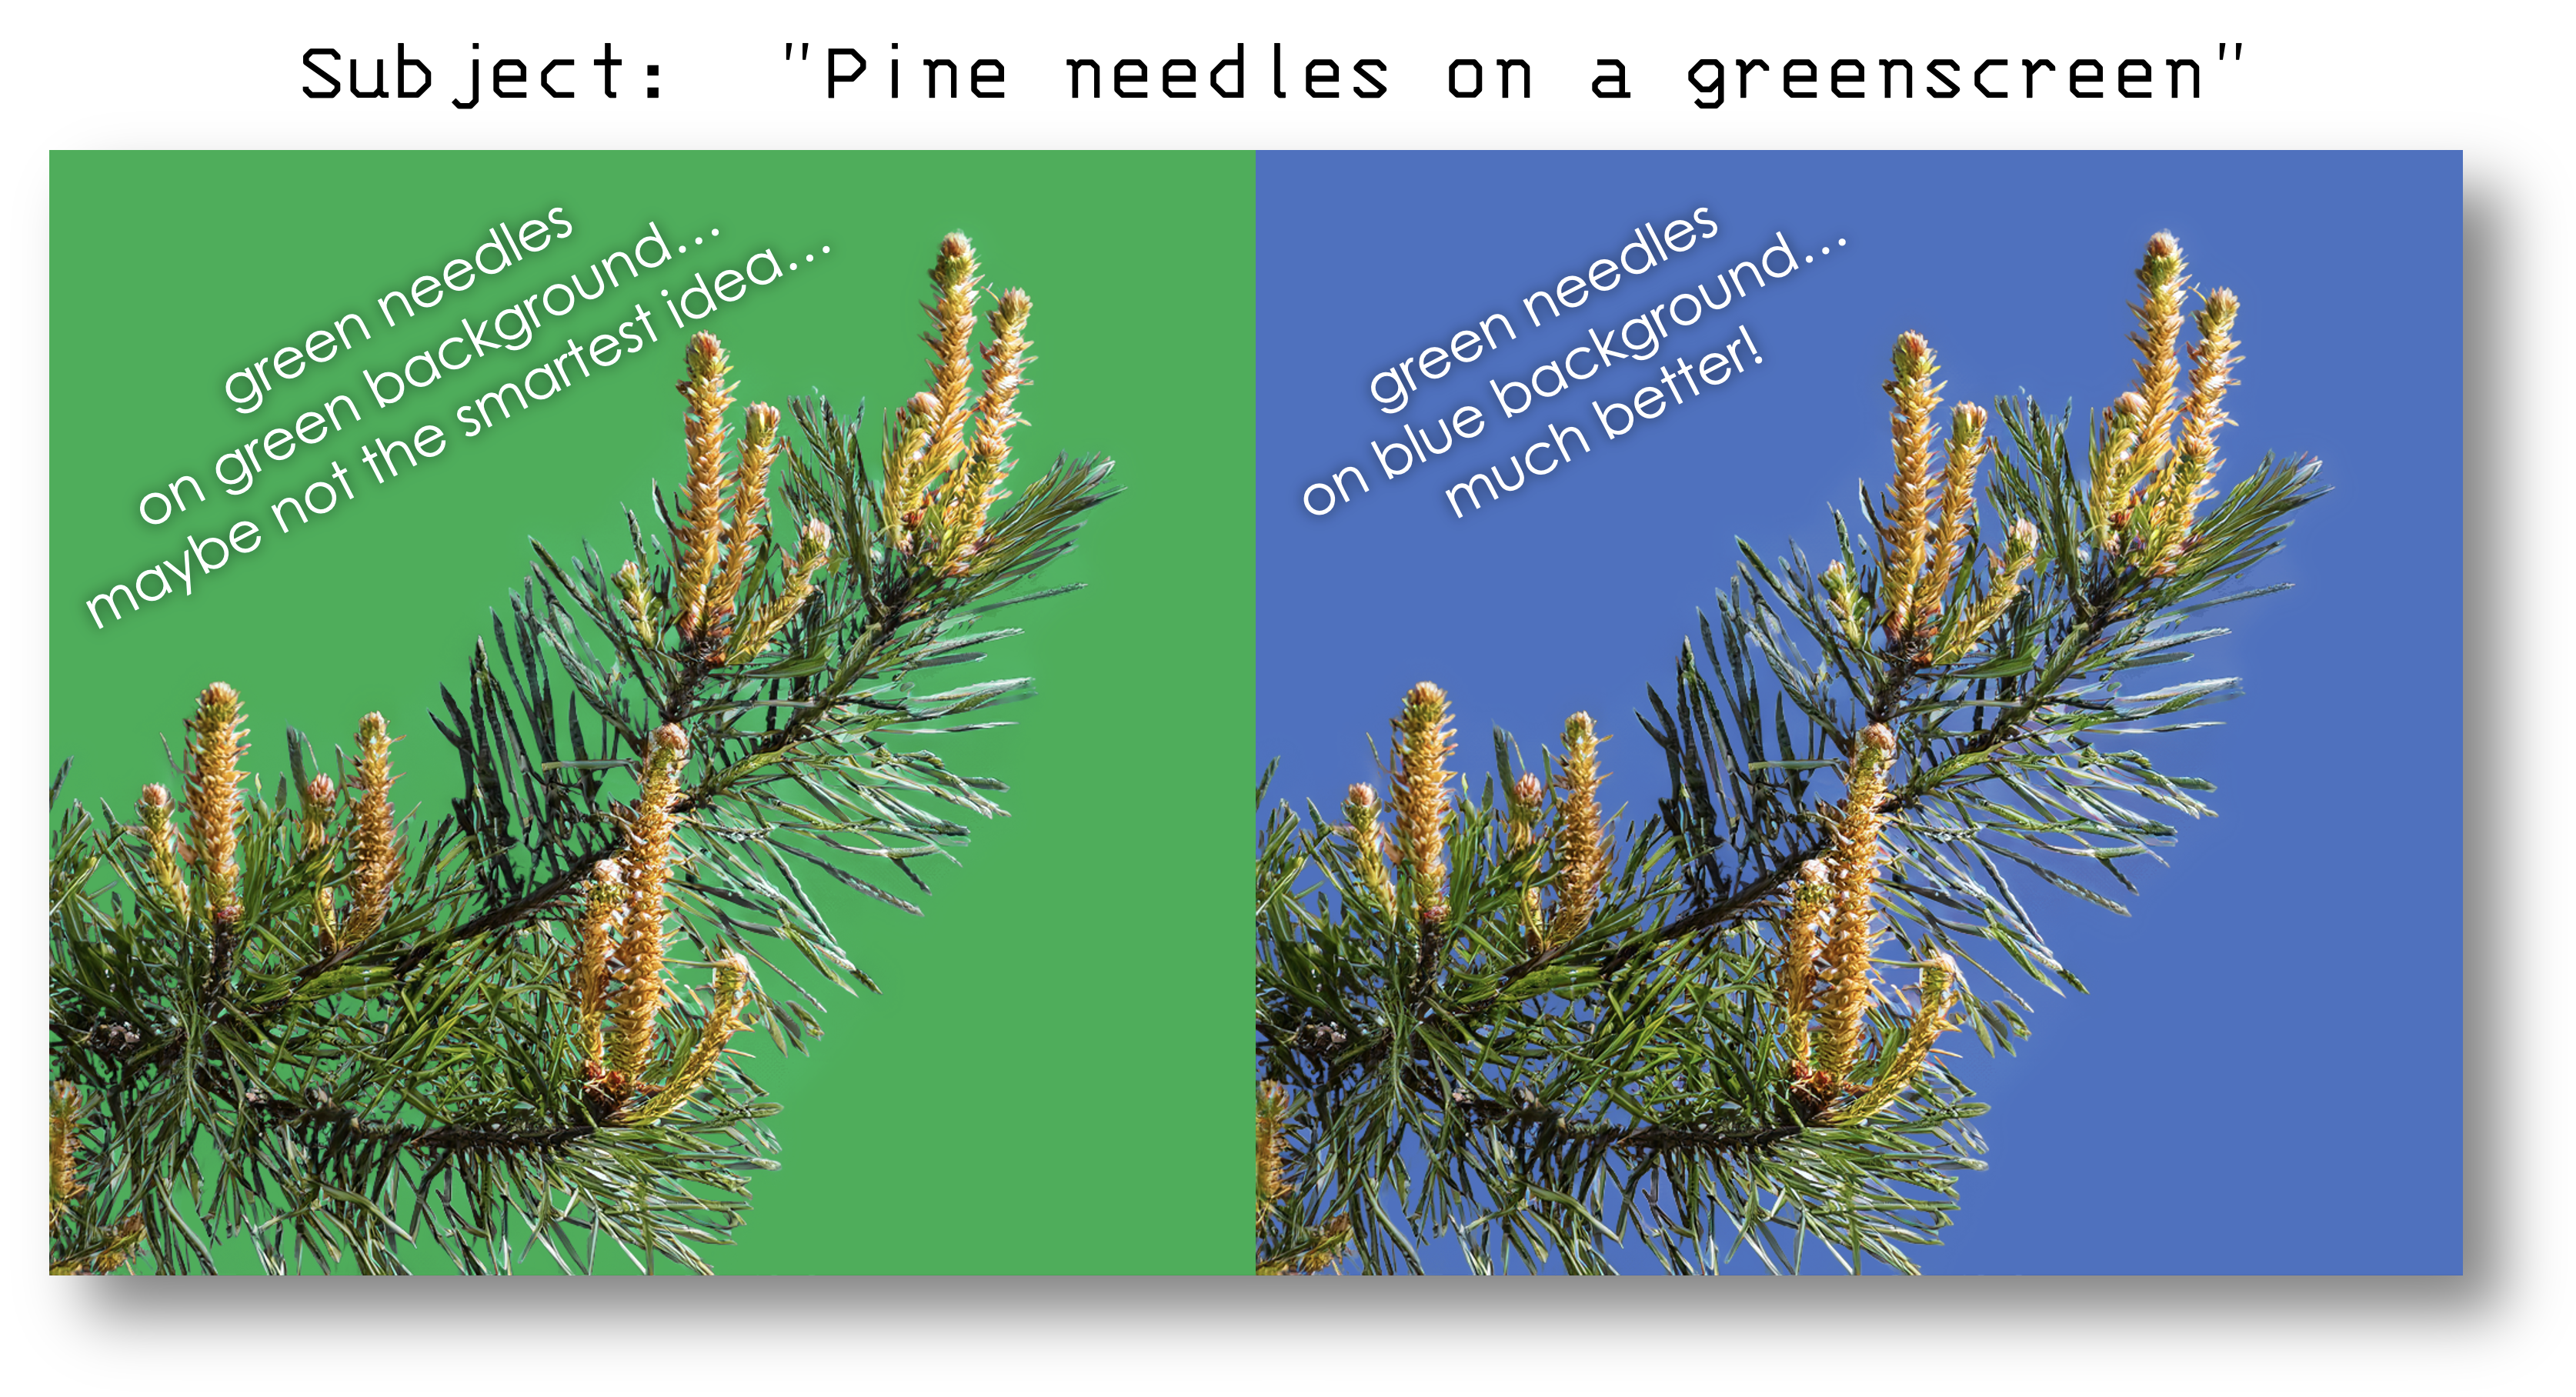
\includegraphics[width=.6\linewidth]{figs/GreenOnGreenBadGreenOnBlueGoodWithShadow.png}
    % 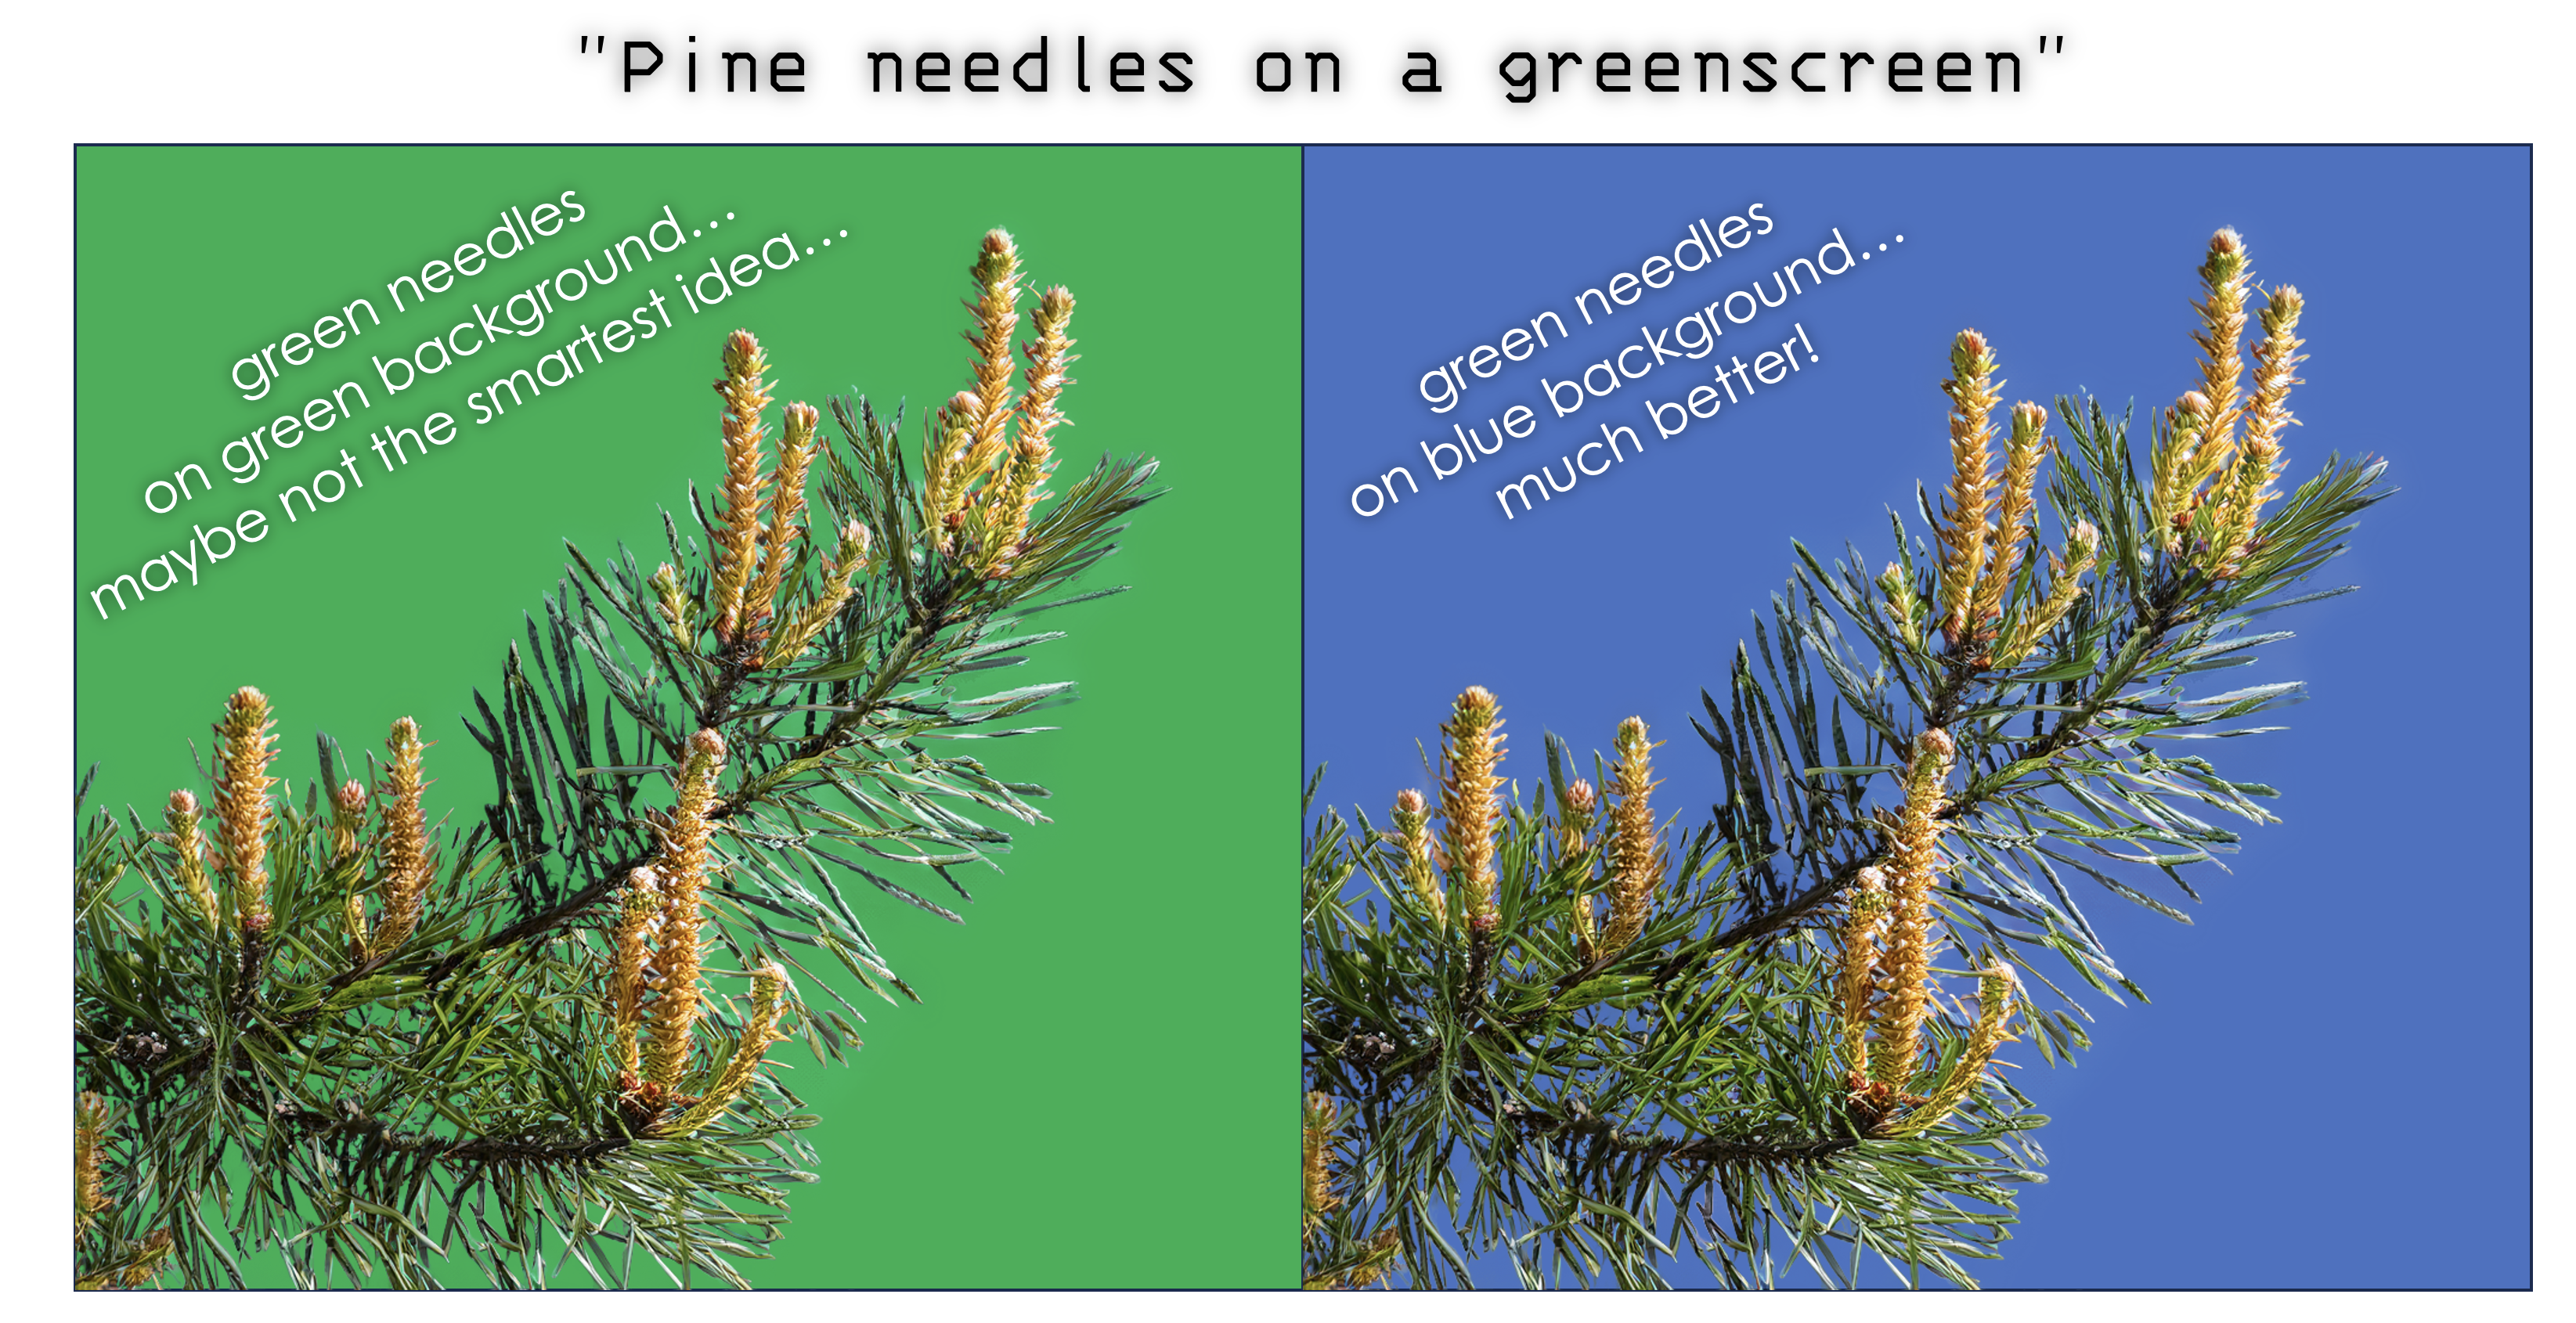
\includegraphics[width=1\linewidth]{GreenOnGreenBadGreenOnBlueGood.png}

    \vspace{-12pt}
    \caption{We need to choose the best background for a given subject, in this case pine needles. To do this, we find the least common hue of the subject.}
    \label{fig:greenOnGreenBadGreenOnBlueGood}

    \vspace{-15pt}
\end{figure}
\end{comment}

\begin{figure}
    %SOURCE: https://stonybrook365-my.sharepoint.com/:p:/g/personal/ryan_burgert_stonybrook_edu/EaPmBbDq3PhAsbIcrfnQirMBGPkeCUVFZLq2y2q5Vb8Nsw?e=4L9bbf
    \centering
    \includegraphics[width=1\linewidth]{figs/LeastCommonHueHistogram.png}
    \vspace{-25pt}
    %\caption{To find the least common hue of a given subject, we first generate an image of that subject with SDXL, then create a histogram of the hues of that image weighted by their saturations. We then smooth the hue histogram with a gaussian kernel with $\sigma=10^\circ$ and take its \textit{argmin}, which is mapped to a string representing that hue (in this case, ``green''). }
    \caption{Finding the least common hue of a given subject. In this example, ``green'' is least common.}
    \label{fig:leastCommonHueHistogram}
\end{figure}

\begin{comment}
\begin{figure}
    %FOR BRIAN: This graph was generated with python code. To generate your own variant use the following link:
    %SOURCE: https://gist.github.com/SqrtRyan/bfb40468a3b52d0ca5ac5c20105f3ea2
    \centering
    % \includegraphics[width=1\linewidth]{figs/LeastCommonHueDistribution.png} %A taller version of the graph
    \includegraphics[width=1\linewidth]{figs/ShorterLeastCommonHueDistribution.png}
    \vspace{-20pt}
    \caption{Green backgrounds and blue backgrounds are by far the most common backgrounds used in our dataset, followed by magenta and rarely yellow or red. Green and blue are generally great colors for chroma keying, especially against human subjects.}
    \label{fig:leastCommonHueDistribution}
\end{figure}
\end{comment}



\subsubsection{Generating \emph{Keyable} Images}

Give a subject and a background color, we can now generate an image from which we will extract the alpha. For this to work, the image must be \emph{keyable}. For an image to be \emph{keyable}, it 1) must have a constant, bright, saturated background color, 2) must not have any objects or gradients in the background, 3) must have fine details like hair, fur, and transparencies in the object when appropriate, and 4) must not have color spill, or background colors tinting the foreground.

Unfortunately, all the publicly available methods we tested were incapable of consistently creating \emph{keyable} images. As shown in Fig.~\ref{fig:greenscreenComparison}, SDXL, Midjourney, Dalle, and Stable Diffusion often produce backgrounds that are not suitable for extraction (being too dark, desaturated, or having gradients or objects) or have color spill. DeepFloyd is quite good at generating vibrant clean backgrounds and foreground with no color spill but fails to produce soft edges (see the lion's mane in~\cref{fig:greenscreenComparison}).

Because of these shortcomings, we propose combining multiple generation methods (namely DeepFloyd and SDEdit) with the goal of overcoming these weaknesses through the combination. Our process is described below.

\begin{figure}
    \centering
    %SOURCE: https://stonybrook365-my.sharepoint.com/:p:/g/personal/ryan_burgert_stonybrook_edu/EVjIIwEUNhdCoA6zD__Cie0BlO27CSHvGBNnDm5eRpXhwA?e=q8zRaJ
    \includegraphics[width=1\linewidth]{figs/priorcomparison.png}
    \vspace{-20pt}
    \caption{We compare results from multiple diffusion models. Each algorithm produces images that are not \emph{keyable}, either the foreground has no fine detail or is tinted green or the background is not suitable for chroma keying. Please zoom in for details.
    }
    %In our testing, only DeepFloyd and Firefly are able to correctly isolate subjects on solid color backgrounds. The background color in SDXL and Stable Diffusion 1.5 are either not green, or too desaturated to perform chromakeying. Note that even though the backgrounds made with SDXL, Midjourney and Dalle are green, they also made the subject green - making it extremely difficult to separate the foreground via chromakey, a problem shown in \cref{fig:greenOnGreenBadGreenOnBlueGood} }
    \label{fig:greenscreenComparison}
\end{figure}

\vspace{-4mm}
\paragraph{Prompt engineering}
We first augment the subject to indicate the background color. For example, if the background color were ``green'', we augment the subject with the phrase \promptstyle{isolated on a solid green background}. 

\vspace{-4mm}
\paragraph{Image generation}
To create a \emph{keyable} image, we use both the text-to-image generation method DeepFloyd followed by the image-to-image generation methods SDEdit. This process is illustrated in \cref{fig:imgToImgPipeline}.

First, we use our prompt with DeepFloyd to generate an initial image. We found that DeepFloyd could consistently produce suitable backgrounds but the foregrounds were lacking detail in the alpha. However, the backgrounds are often not as bright and saturated needed for SDEdit. To address this, we perform an initial extraction of the object and composite it onto a brighter, more saturated background with the approximately same hue. We use Photoshop's Subject Selection feature, a method that uses deep-learning-based segmentation and matting to compute masks for primary objects in an image and can be run in batch mode.  This method does not perfectly extract the object and may leave green pixels in regions like hair, but these typically do not cause a problem as the object is immediately composited onto a similar colored background.

We then use SDEdit \cite{sdedit}, the image-to-image version of SDXL implemented by Huggingface \cite{huggingface_img2img}, to regenerate the final image.  In this step, we need to guarantee that the object has fine details, that it has no color spill, and that the background is solid, bright, and saturated enough for chroma keying. To produce fine details, we set SDEdit's strength parameter to .95. This parameter, ranging from 0 to 1, determines how closely the generation follows the input image by modulating the amount of noise added to the image. This allows enough freedom for SDEdit to generate a new version of the same object with better details, not only at the edges but often in the interior of the object as well. To prevent color spill, we add the background color as a negative prompt. This suppresses that color in the foreground object, but because the background is so bright and saturated from the previous step it fails to suppress the color in the background. 

\cref{fig:beforeAfterImg2Img} shows the impact of this process. The images in the column ``Before Img2Img'' are the outputs from DeepFloyd after being matted by Photoshop Subject Selection and composited onto a solid background, and the ``AfterImg2Img'' column are the outputs of SDEdit. Note the fidelity of the image increases and any color spill corrected due to the negative prompt. (e.g. the submarine's green tint or the girl's green dress). Also note the mistakes made by Photoshop Subject Selection are corrected as well - the dandelions look poorly extracted before SDEdit but look natural after.

Despite these efforts to make the images as \emph{keyable} as possible, our process is imperfect, sometimes yielding results with gradients in the background color or tinting of the foreground object. To deal with this, we require a robust alpha computation method.

\begin{comment}
\bp{There are a lot of figures with oversized captions - could you please move those long captions into the body of this section and condense it down? Thank you!}

[The description of the pipeline in the figures 
\cref{fig:imgToImgPipeline}
\cref{fig:geishaComparison}
\cref{fig:beforeAfterImg2Img}
is enough to fill out this section, with the additional information below]

We use a strength of .95 with img2img [cite SDEdit again which should be in related works], and our negative prompt is 'green'. The reason it still has a green background after this step is because of the compositing step we did with Foreground Selection Blended onto green background. That step makes the background saturated enough that even at a strength of .95, img2img still won't change it. This allows us to make dramatic improvements to the image with img2img, seen in the figure \cref{fig:beforeAfterImg2Img}. If we didn't use img2img, we couldn't use 'green' in the negative prompt, and we would have to deal with more frequent greenspill issues. @Brian this is the trick that lets us get so much of the dataset via automatic selection (up to 50\%) vs the original firefly one (maximum 25\%, probably should be more like 15\% if you're going to play it safe). 
\end{comment}



\begin{figure}
    \centering
    %SOURCE: https://stonybrook365-my.sharepoint.com/:p:/g/personal/ryan_burgert_stonybrook_edu/EVjIIwEUNhdCoA6zD__Cie0BlO27CSHvGBNnDm5eRpXhwA?e=q8zRaJ
    \includegraphics[width=1\linewidth]{figs/img2img_pipeline.pdf}
    \vspace{-20pt}
    \caption{We generate the RGB images in our dataset using a combination of both DeepFloyd, Photoshop's Subject Selection feature, and Stable Diffusion XL. The resulting images have near-perfect, high saturation backgrounds that are ideal for chroma keying. Please zoom in for details.}
    \label{fig:imgToImgPipeline}
\end{figure}




\begin{figure}
    %SOURCE: https://stonybrook365-my.sharepoint.com/:p:/g/personal/ryan_burgert_stonybrook_edu/EVjIIwEUNhdCoA6zD__Cie0BlO27CSHvGBNnDm5eRpXhwA?e=q8zRaJ
    \centering
    % \includegraphics[width=.5\linewidth]{figs/BeforeAfterImg2Img.pdf} %This one is tall
    \includegraphics[width=1\linewidth]{figs/BeforeAfterImg2ImgFlat3.pdf} %This one is flat
    \vspace{-20pt}
    \caption{Examples of image before and after applying image-to-image SDEdit. The before images are outputs of DeepFloyd after being extracted by Photoshop Subject Selection and composited onto a new background. Please zoom in for details.}
    \label{fig:beforeAfterImg2Img}
\end{figure}

\subsubsection{Alpha extraction} 

Once we have a \emph{keyable} image, we must extract the alpha from the image. Unfortunately, this is also a difficult process. Chroma keying is an underconstrained problem. Even with a solid background color, chroma keying methods can fail to correct compute the alpha, and in practice users must manually change parameters or correct the mattes for a high quality result. This time-consuming process does not scale to large datasets.

To address this, we generate three alpha mattes and choose between them. These three methods operate differently and in difficult cases one algorithm may compute accurate results when the other cannot.
The algorithms we use are: 
\\
1. \textit{A pixel-based chroma key method}. We modified a traditional color difference chroma key algorithm~\cite{wright2010taylor} that takes a single rgb color representing the background as input to instead take a background rgb color per pixel. We conservatively delete the foreground object and inpaint the background using \cite{Telea2004}  to provide the background color at each pixel. This allows us to better handle subtle gradients in the background color. Note that this also performs color decontamination in the same step.
\\
2. \textit{A deep-learning based chromakey model} that was trained on an internal dataset and takes in an input RGB image and a background RGB image and returns the alpha and foreground color. 
\\
3. \textit{Photoshop's Subject Selection} which uses proprietary segmentation and matting algorithms to select the primary object in an image. It works well on images with simple backgrounds and is robust to color spill.

\cref{fig:alpha_compare} compares the three methods on three examples, highlighting cases where the methods have inconsistent results. In such cases, one of the methods is able to compute an accurate alpha.

\begin{comment}
\bp{Sorry that this is so messy...I put down all the information we need though}

\bp{[Figure:Show Where each succeeds and where each fails. Examples can be found in the exit talk powerpoint presentation, or gathered from the URL with the dataset - just disable the algorithsms you don't want to see and you can even screenshot them all at once]}

The backgronud color is estimated in a process you can see in the exit talk powerpoint (link to it is in slack), though we might just skip talking about that here and put it in the appendix. The gist is: we do floodfill from the corners of the image, and then inpaint the background to erase the foreground and use that as the background image for chromakeying.


We have three \textit{primary} matting algorithms: 
\\
1. \textit{A pixel-based chromakey algorithm} which maps ( RGB  pixel from image + RGB keying value from background image) to (RGBA output pixel). Note that this also performs color decontamination all in the same step.
\\
2. \textit{A deep-learning based chromakey model} that was trained on an internal dataset and takes in an input RGB image + a background RGB image and retuns an outputted color-decontaminated RGBA image. 
\\
3. \textit{Photoshop's Subject Selection }(which is robust to the background color and robust to any greenspill, and which can perform matting but almost always fails on glass, and is a lower resolution than the others). It also operates at a lower resolution than the other methods, and doesn't capture as much detail.

\end{comment}

Recalling the image matting equation:
\begin{equation}\label{eq:compositing_equation}
  I = \alpha F + (1-\alpha) B,
\end{equation}
we require not just the alpha but also $F$, the pure foreground color of the pixel with any background color $B$ removed. Each of our three alpha extraction methods generate a predicted $F$. However, the method that predicts the best alpha does not necessarily also produce the best $F$. Experimentally, we chose the best seven combinations as possible choices for the final alpha and $F$.


\begin{figure}
    \centering
    % 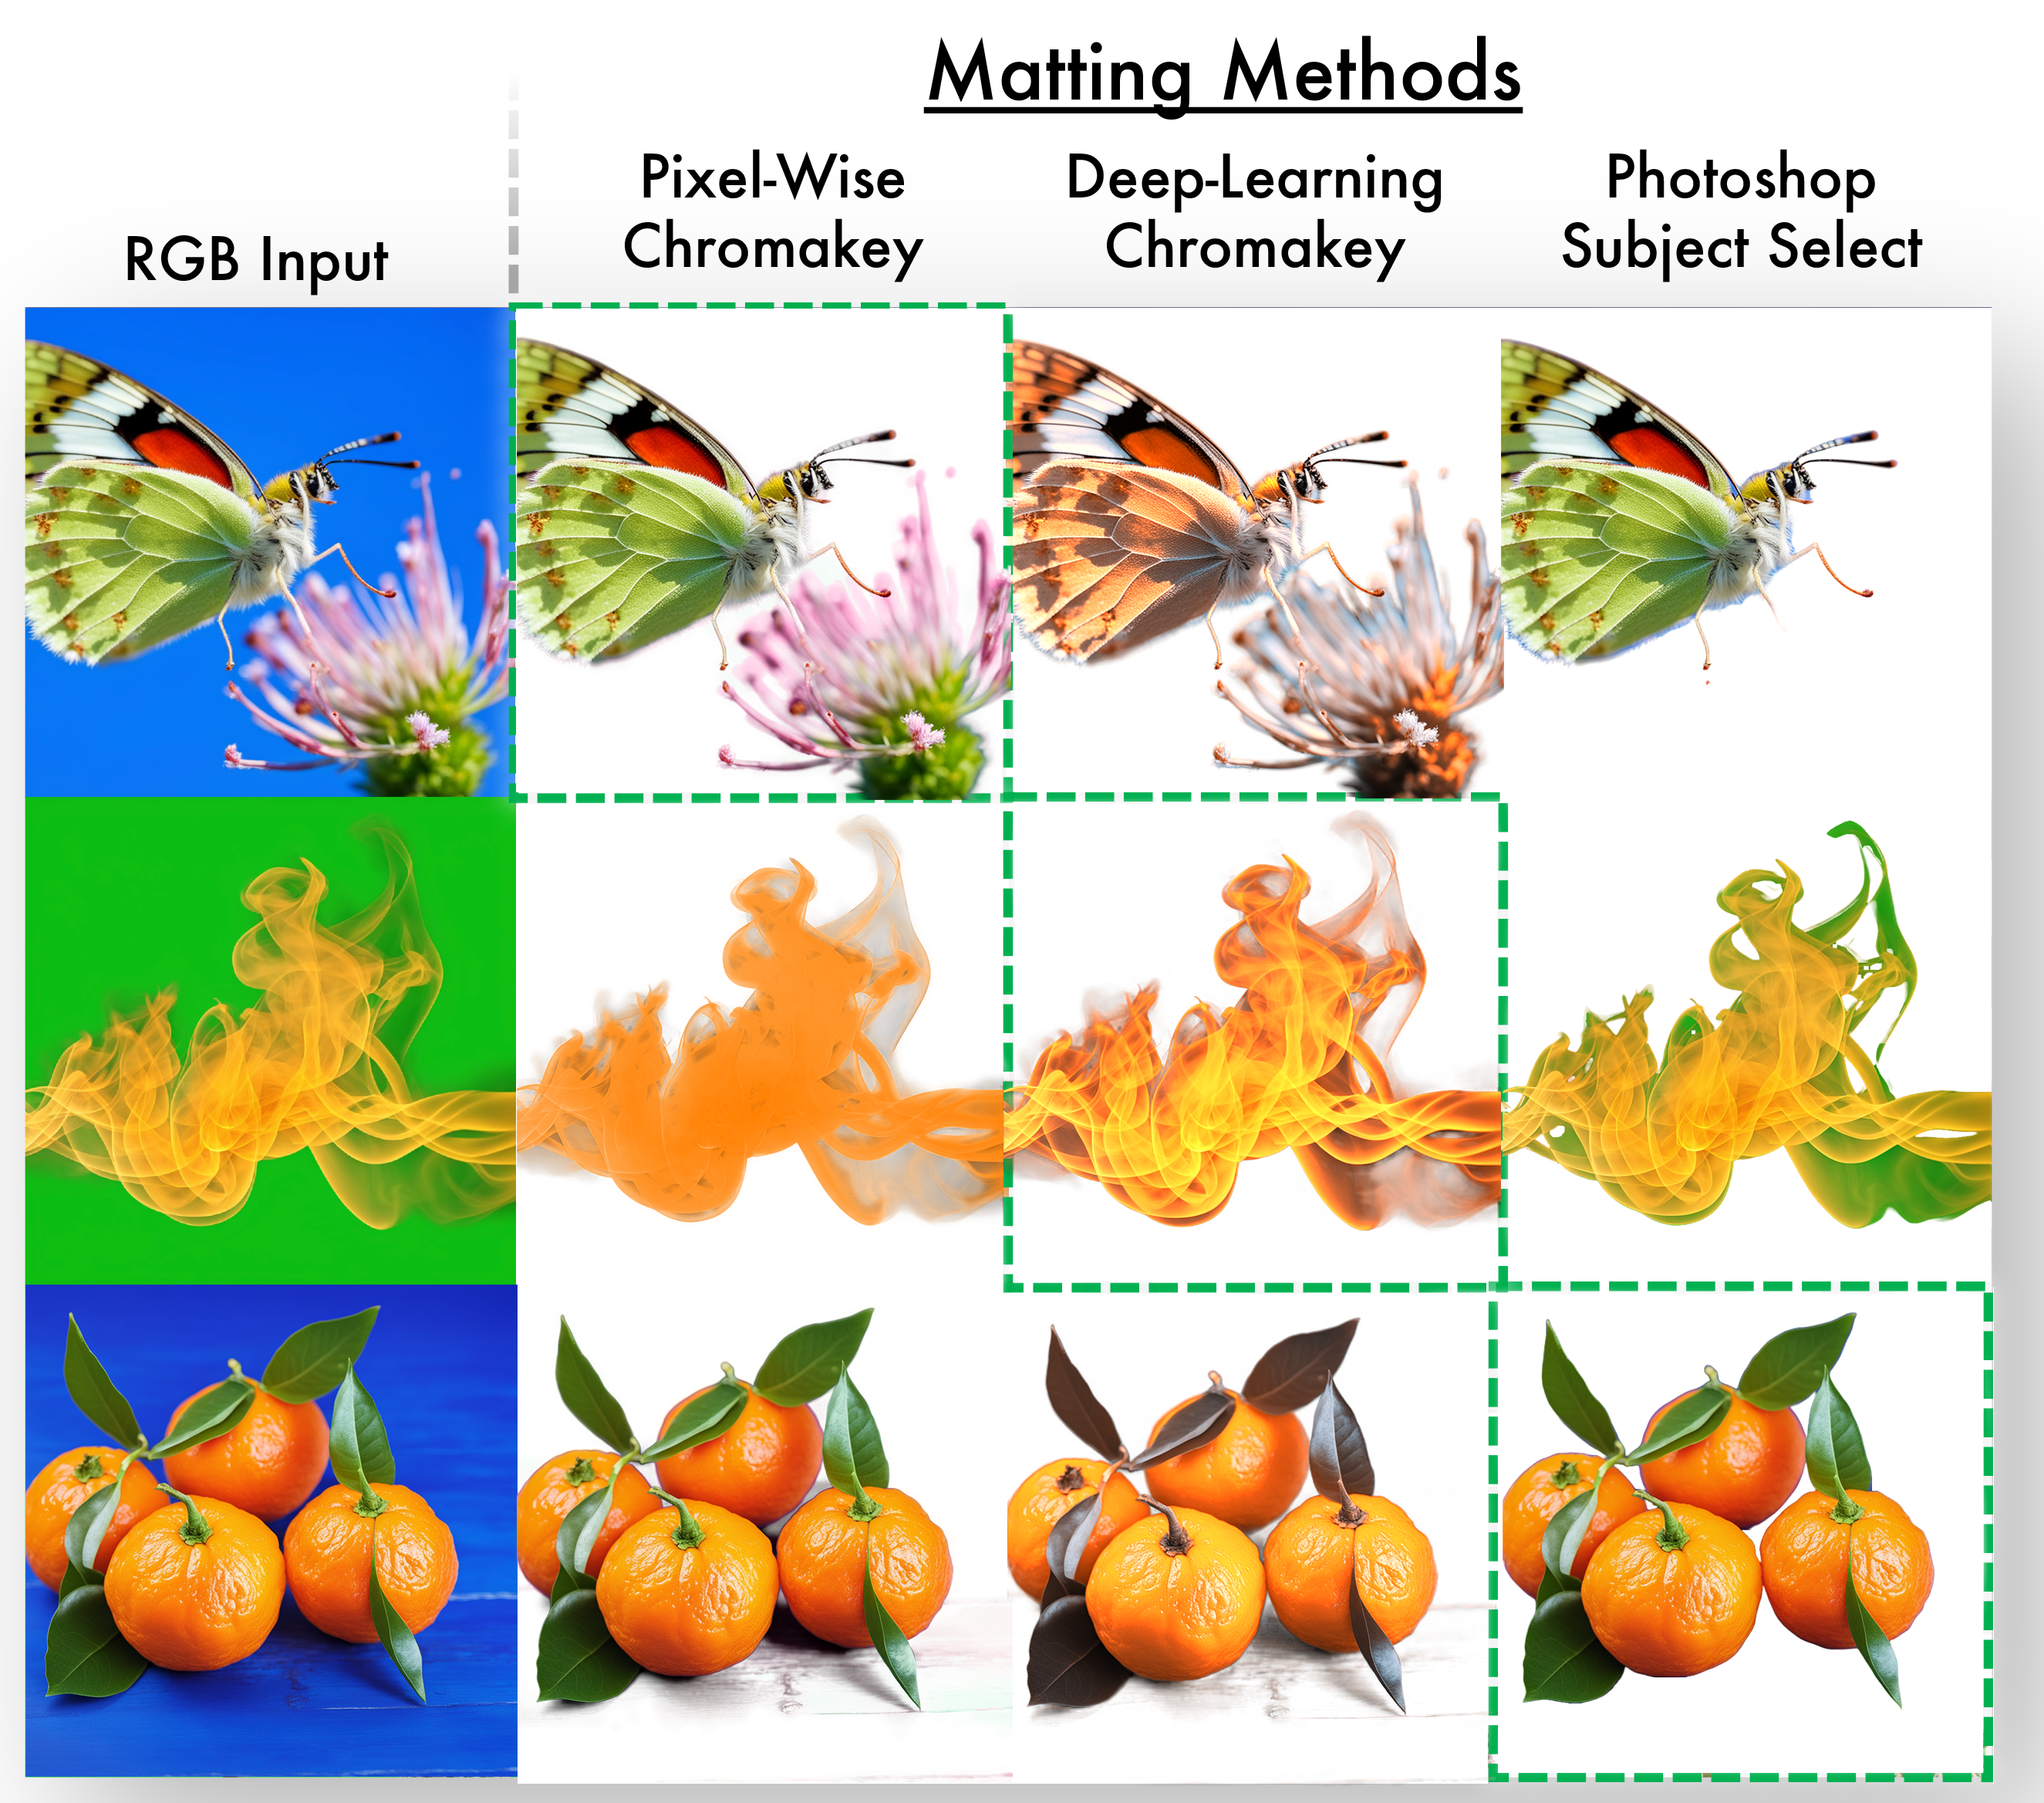
\includegraphics[width=1\linewidth]{figs/MattingMethods.pdf}
    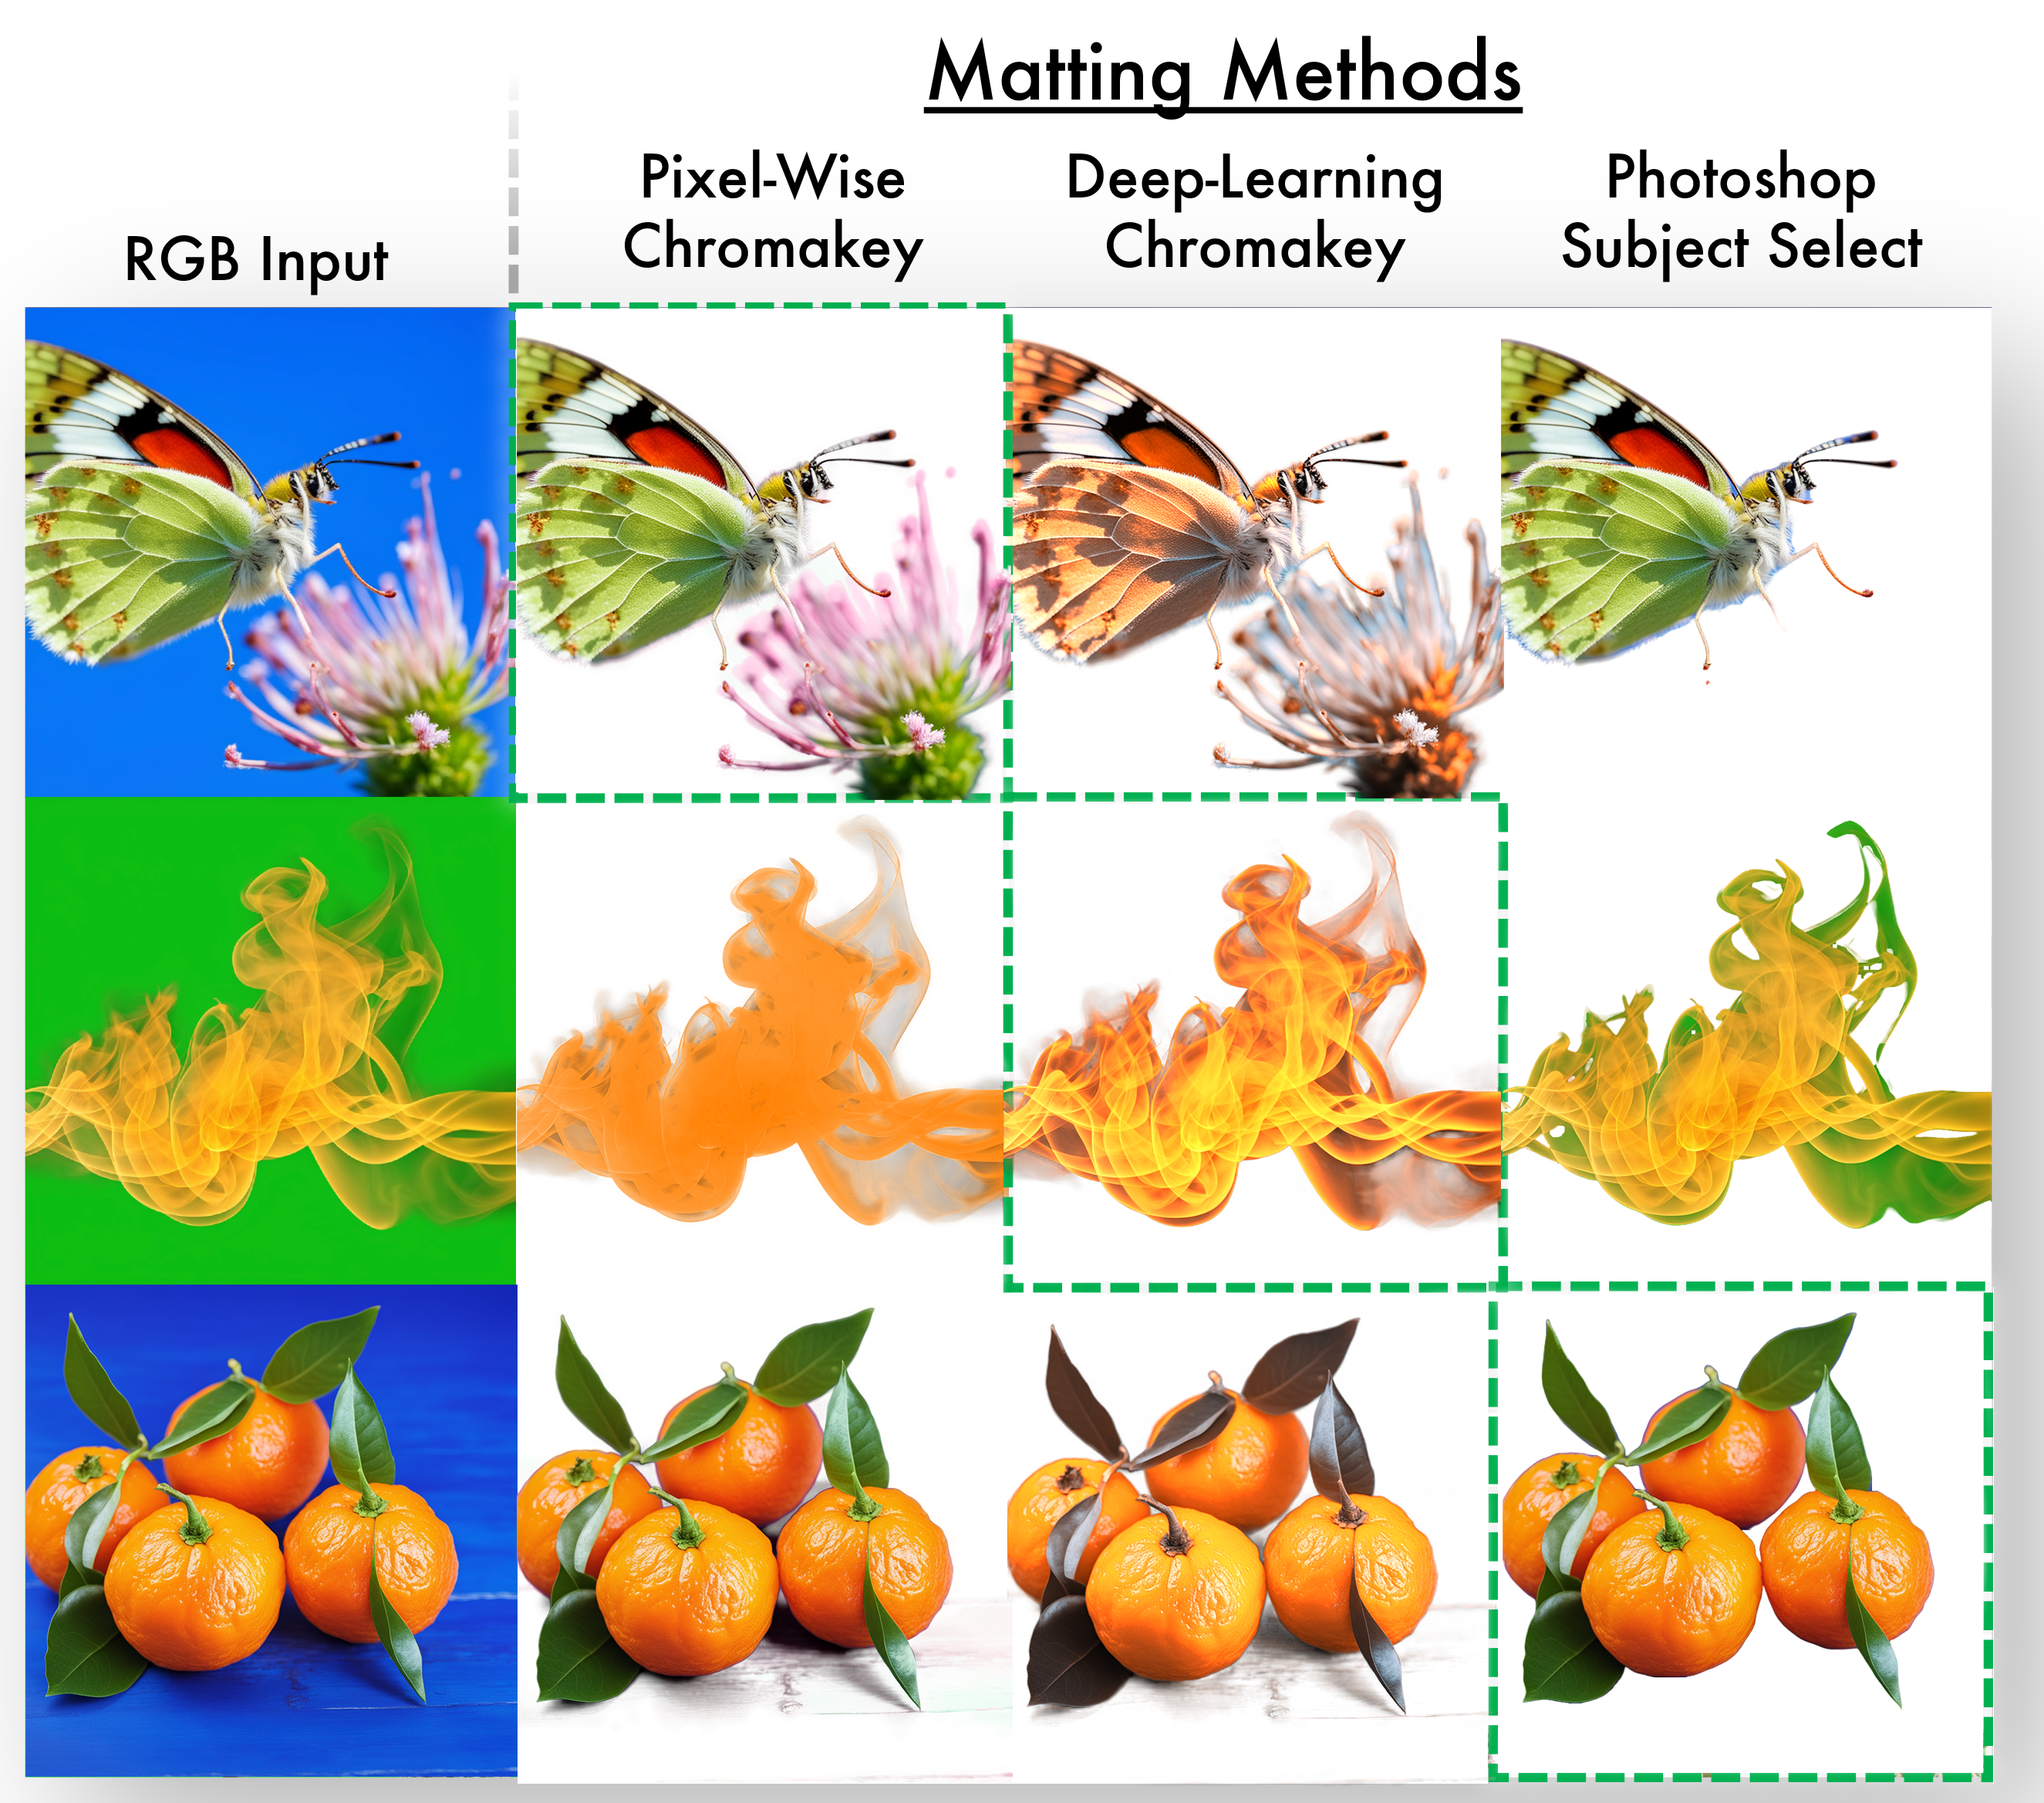
\includegraphics[width=1\linewidth]{figs/MattingMethods.png} %Renamed it Primary matting methods to emphasize that it's not the derived mix-match ones
    \vspace{-20pt}
    \caption{A comparison of our three matting methods on different input images. The green dotted rectangles indicate the best result for each example.  
    %The image in the last row normally won't have any green because of the negative prompt in the img2img step - but for the sake of this illustrative example to highlight where photoshop subject select does well I put it in there anyway. Note that the derived mix-match matting methods where we mix rgb/alpha from different primary methods are not shown here 
    %\bp{-- subject select is very rarely the correct choice in this dataset, whereas in the firefly dataset it was relatively common. Its main use is for the similarity score metric for auto-selection, for which it is a critical component}.
    }
    \label{fig:alpha_compare}
\end{figure}



\subsubsection{Image Selection Process}
\label{sub:image_selection_process}
The last step in our dataset creation pipeline is to select the best matte. Each subject will have multiple matted results, and the goal of this step is to choose the best one. We propose a simple automatic process that can approve a large number of the images. For those failing the automatic process, we fall back to having humans select the best option.

\vspace{-4mm}
\paragraph{Automatic Selection Process}
Each of our alpha extraction methods operate differently, with one being color-based, one being trained for computing alpha from greenscreen images, and one being designed for general object extraction. Because of this, they tend to make different mistakes. However, for cases where our method successfully produced a \emph{keyable} image, the three alpha extraction methods often produce nearly identical results. We use this as an indication that the alpha computation was successful and each of the resulting alphas are good.

To measure the similarity, we devise a similarity score metric taking into account both their alpha and RGB values - but not penalizing differences in RGB values if the alpha values are both low. To do this, we compare both RGBA images composited on different backgrounds (white and black) and take the mean similarity between these two composite images. We measure this similarity using MSSSIM~\cite{MSSSIM} (multi-scale structural image similarity) as we found it gave the best results empirically. 

MSSSIM is a metric that measures similarity between images on a scale from 0 to 1, assuming the pixel values are also between 0 and 1. Given our three RGBA images $I_0$, $I_1$, and $I_2$, a white image $W$, a black image $B$, the composition function $\mathcal{C}$ and the MSSSIM function $\mathcal{M}$, we compute our similarity score $\mathcal{S}$ as:
\begin{equation}
\begin{split}
    \mathcal{S} = min_{(a,b)} \mathcal{F}(I_a, I_b) \text{\ \ \ where\ } a,b \in \{0,1,2\}  \\
    \mathcal{F}(I_a,I_b) = \frac{1}{2} (  \mathcal{M}[\mathcal{C}(I_a,W),\mathcal{C}(I_b,W)] \\ 
                            + \mathcal{M}[\mathcal{C}(I_a,B),\mathcal{C}(I_b,B)] )
\end{split}
\end{equation}
\cref{fig:simility_comparison} shows a visual comparison between images with a high and a low similarity score.

\begin{comment}
{
\footnotesize
$\text{rgba\_similarity}(image\_a, image\_b) = \frac{1}{2} \left( \text{MSSSIM}(\text{composite}(image\_a, \text{white}), \text{composite}(image\_b, \text{white})) \right. \\
+ \left. \text{MSSSIM}(\text{composite}(image\_a, \text{black}), \text{composite}(image\_b, \text{black})) \right)
$

$\text{similarity\_score}(images) = \min_{(a, b)} \text{rgba\_similarity}(a, b) \quad \text{where} \quad (a, b) \in images \times images
$
}
\end{comment}

\cref{fig:similarityScoreHistogram} shows the distribution of similarity scores. Most images have very high similarity scores, indicating our process to make the images \emph{keyable} was largely successful. The median score is 0.984. We found that the top 50\% of samples (measured by similarity score) yield decent results, resulting in 110,000 images in our dataset being automatically selected. These objects tend to be solid objects including objects with hair or fur, and tend to not be objects with significant transparencies. For these automatically-selected images, we choose the pixel-wise chroma keying algorithm as it often gives the highest detail.

%The subjects that are selected automatically tend to be solid objects, as opposed to glass - since in order to have a high similarity score, the chromakey algorithm must yield similar results to the Photoshop Subject Selection algorithm, which almost always rounds to 1 on any semi-transarent object, thereby giving glass a low similarity score.

\vspace{-4mm}
\paragraph{Manual Selection Process}
For images that do not fall above the threshold of automatic selection, we rely on humans to select the best alpha for us.  These tend to be subjects that contain difficult transparencies such as glass, water, smoke, or fire. We acquired 40,000 images using manual selection of the computed mattes.

We've created a program that will be released to the public along with our dataset to aid in manual selection. 
%(see Fig~\ref{fig:ui}). 
It presents multiple combinations of alpha and $F$ and allows changing the background colors and zooming for accurate assessment of details, as well as additional features such as tagging images. It also serves as an efficient way to quickly view and audit the dataset. See the Appendix for details.


\begin{figure}
    \centering
    \includegraphics[width=1\linewidth]{figs/sim_score_qualitative2.pdf}
    \vspace{-20pt}
    \caption{A qualitative comparison of a high and low similarity score. Note how the alpha masks and colors are different between samples on the one with low similarity, but nearly identical on the one with high similarity.}
    \label{fig:simility_comparison}
\end{figure}

\begin{figure}
    \centering
    \includegraphics[width=1\linewidth]{figs/simScoreDistribution2.pdf}
    \vspace{-20pt}
    \caption{The distribution of similarity scores in the dataset.}
    \label{fig:similarityScoreHistogram}
\end{figure}


\begin{comment}
\begin{figure}
    \centering
    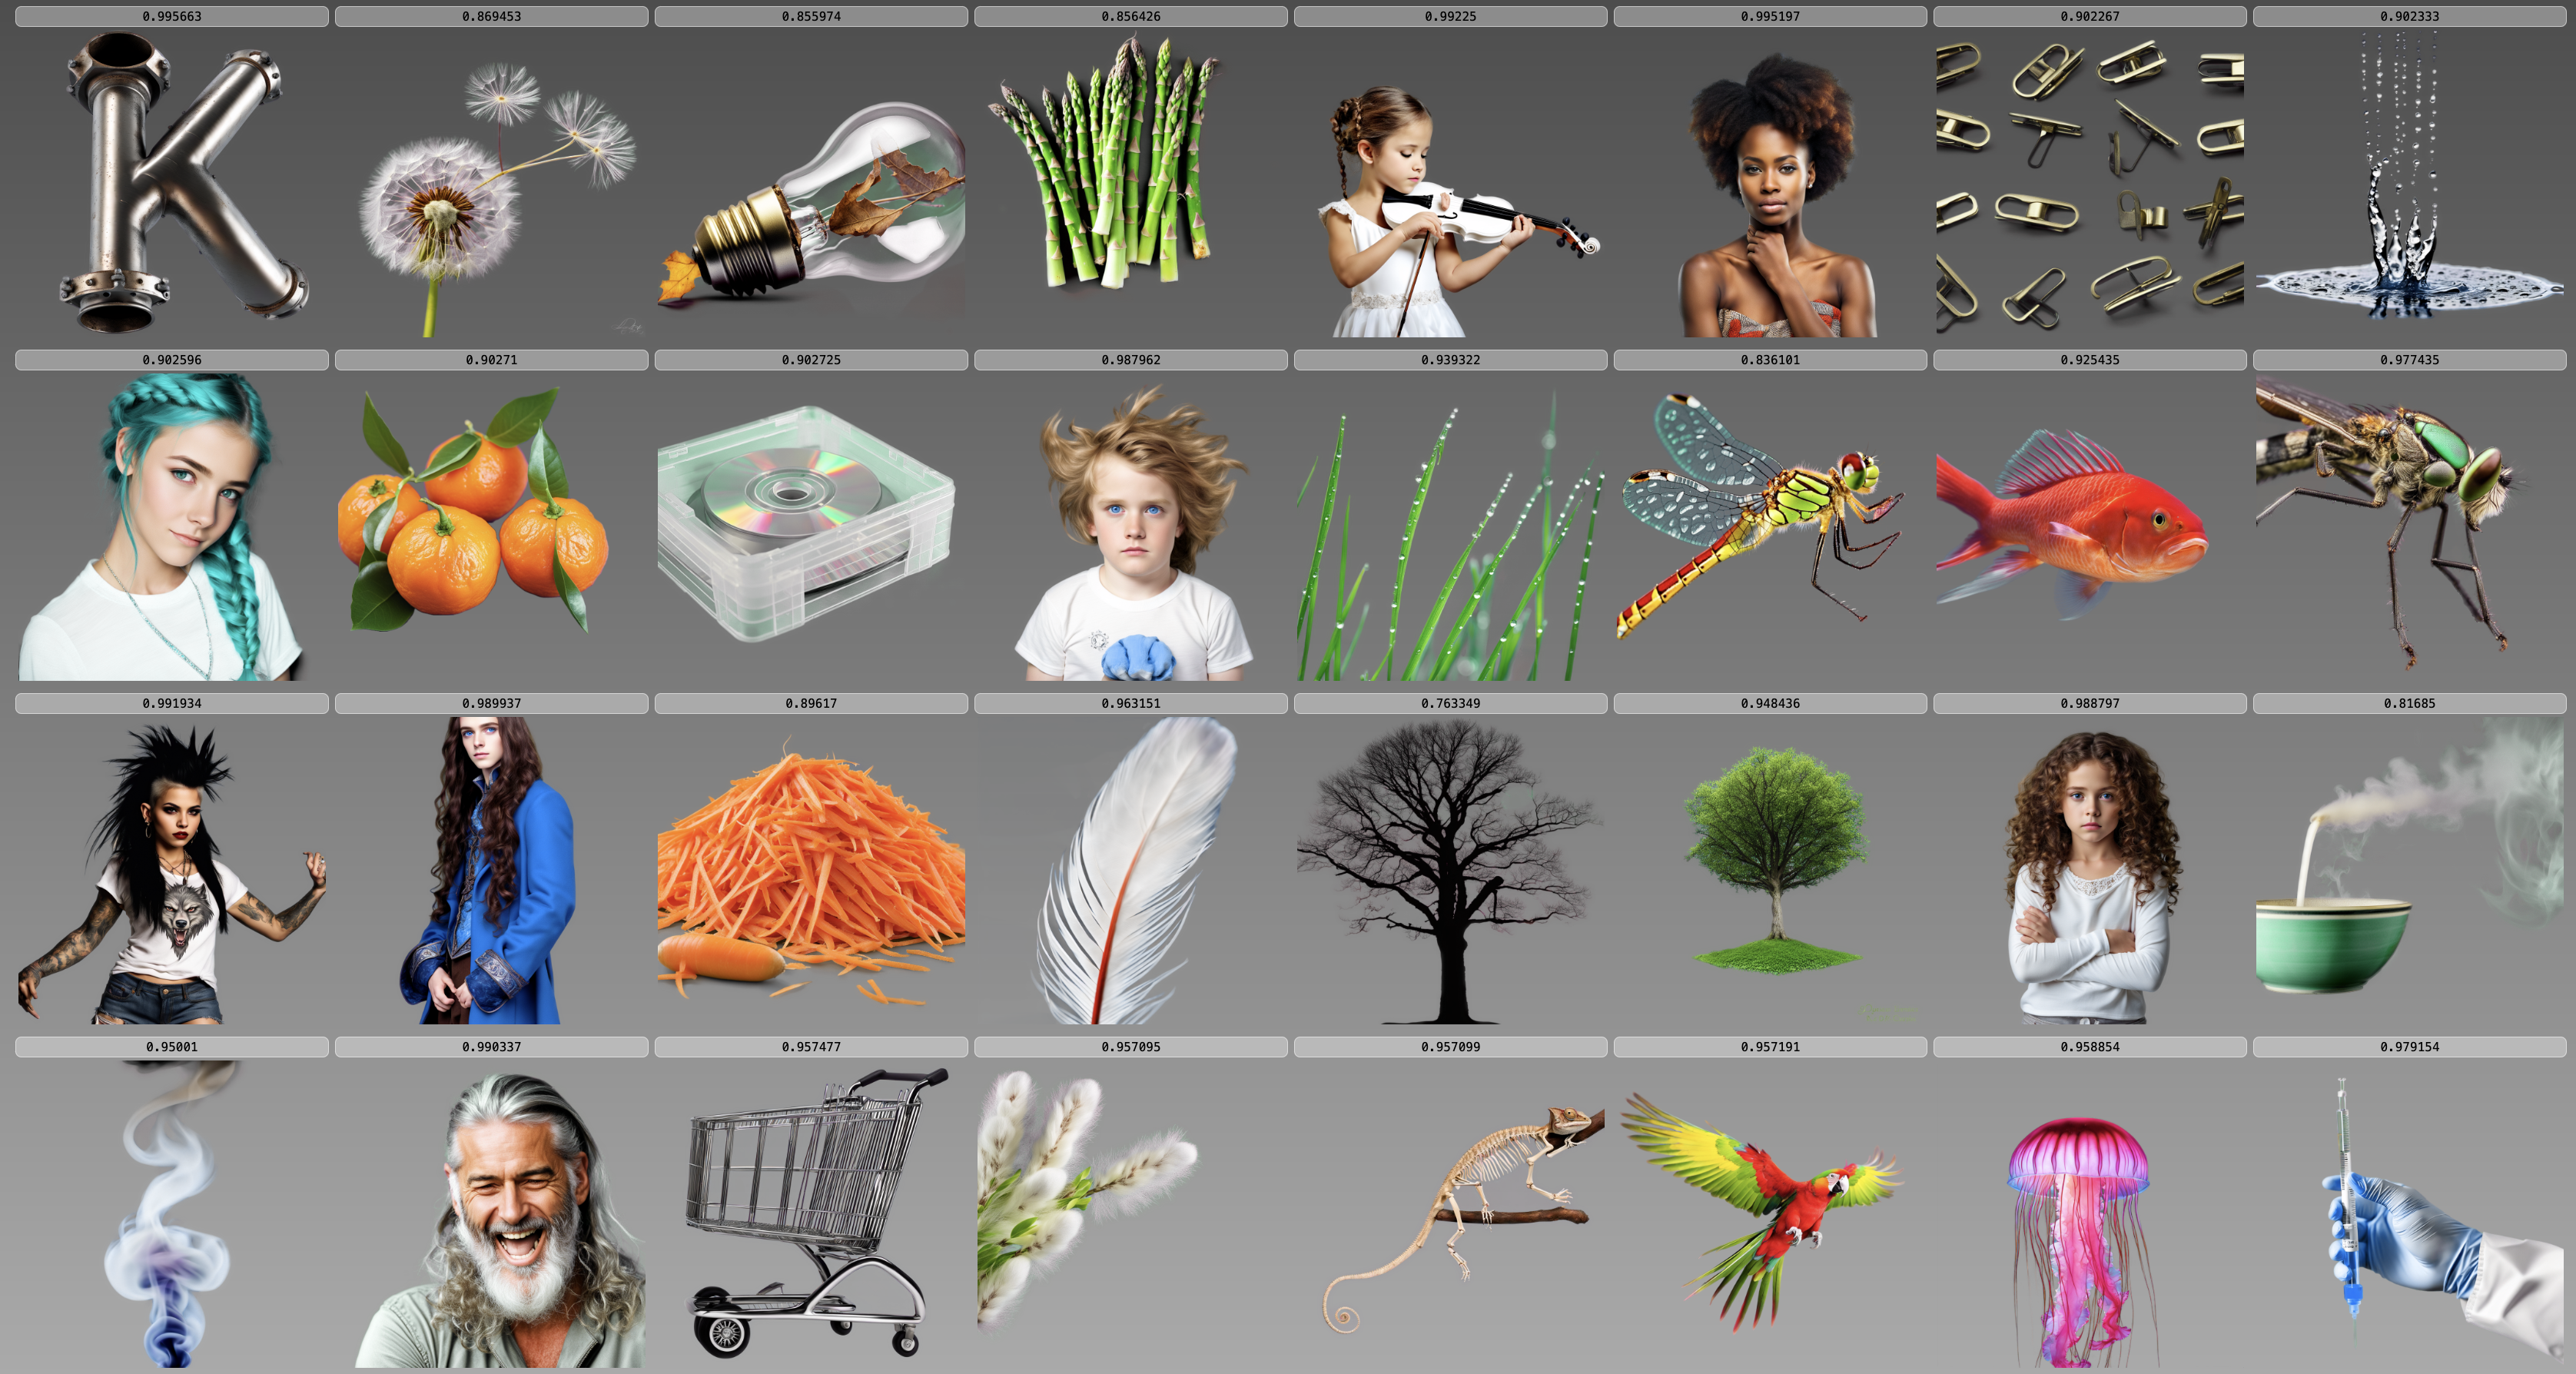
\includegraphics[width=1\linewidth]{figs/moreQualitativeSimilarityScores.png}
    \caption{A subset of the images shown in \cref{fig:datasetExpose}}
    \label{fig:enter-label}
\end{figure}

\paragraph{The Manual Way}

The not automatically way means we pay annotators \$30,000 and wait several months. We did this - and it's a lot cheaper than having people manually matte images in photoshop or gimp etc at a cost of \$0.30 per image. 

We've created a program that will be released to the public along with our dataset that makes annotation very fast. All the annotators have to do is click the best of several images over an over again. It includes many features that are specific to this task, such as being able to quickly switch the background color or view an image's alpha mask with a single keypress. It supports dividing up the workload among several workers, so they can work on the job in parallel. Also, this serves as a good way to quickly view and audit this datasetas it supports several searching features.



\begin{figure}
    \centering
    % \includegraphics[width=1\linewidth]{figs/userInterface.png}
    % \includegraphics[width=1\linewidth]{figs/ui2.png}
    \includegraphics[width=1\linewidth]{figs/ui3.png}
    \caption{A web-based annotation program designed specifically for the task of creating this dataset. Combinations of the alpha and foreground colors from three primary matting methodsare shown in the columns. For each image, the user clicks the best one.}
    \label{fig:ui}
\end{figure}

\end{comment}

\begin{comment}


\subsection{Additional Dataset Statistics}
Our data-set contains both safe-for-work and NSFW content, which is labeled as such. Approximately $.15\%$ of the samples in our dataset are flagged NSFW, as determined by a combination of the human annotators and a check for over 3000 blacklisted keywords present in the subjects. 

Additionally, the dataset contains a mix of shadows and non-shadows - as some samples will include soft shadows in their alpha-matte. 

The whole dataset generation process was accomplushed on 32 A100 GPU's over the span of three weeks, plus an additional two months of human annotation with a budget of \$30000 USD. 

\end{comment}